\appendix
\section{Appendix A} \label{appendixA}


\begin{Figure}
    \centering
    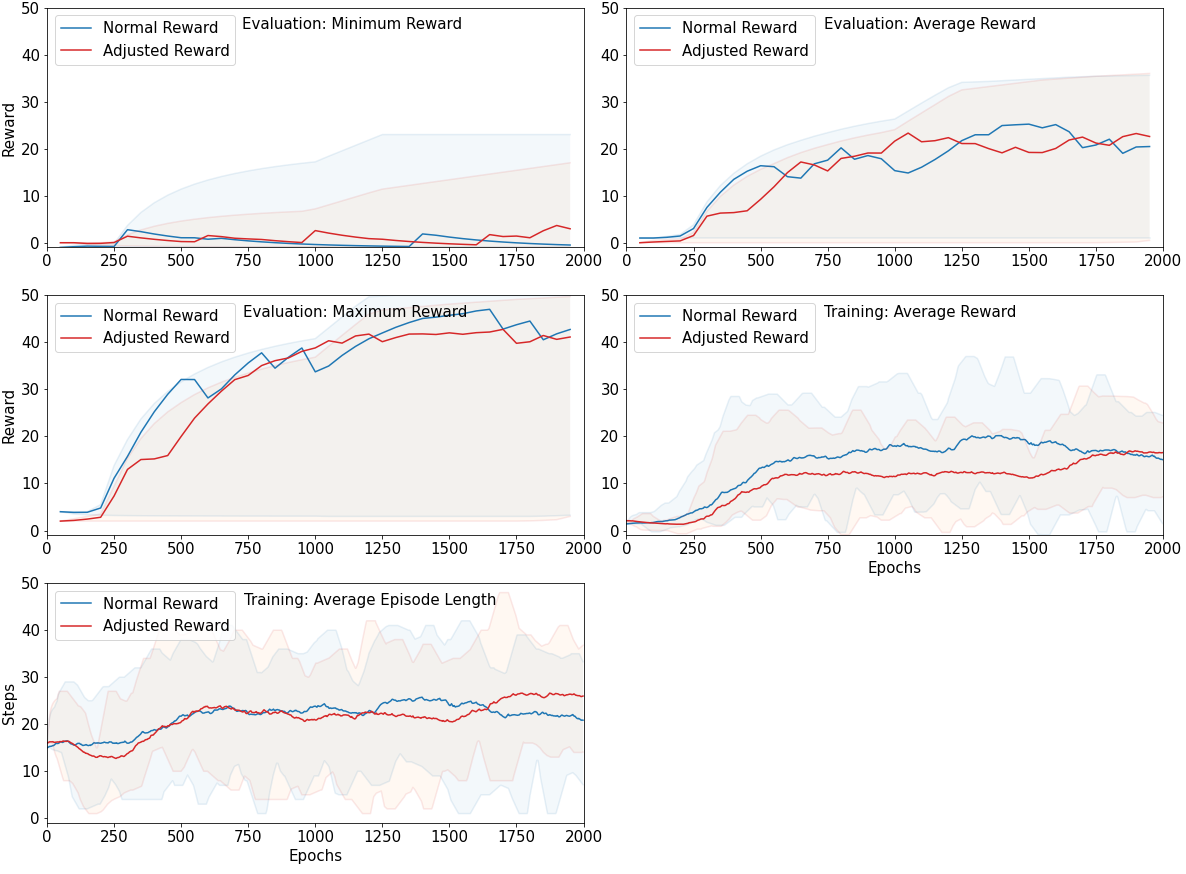
\includegraphics[width=\linewidth]{results/NewReward Training in BlocksObstacles.png}
    \captionof{figure}{Training Process in BlocksObstacles Environment with Adjusted Reward}
    \label{im:NewRewardTraining}
\end{Figure}


\begin{SCfigure}
    \centering
    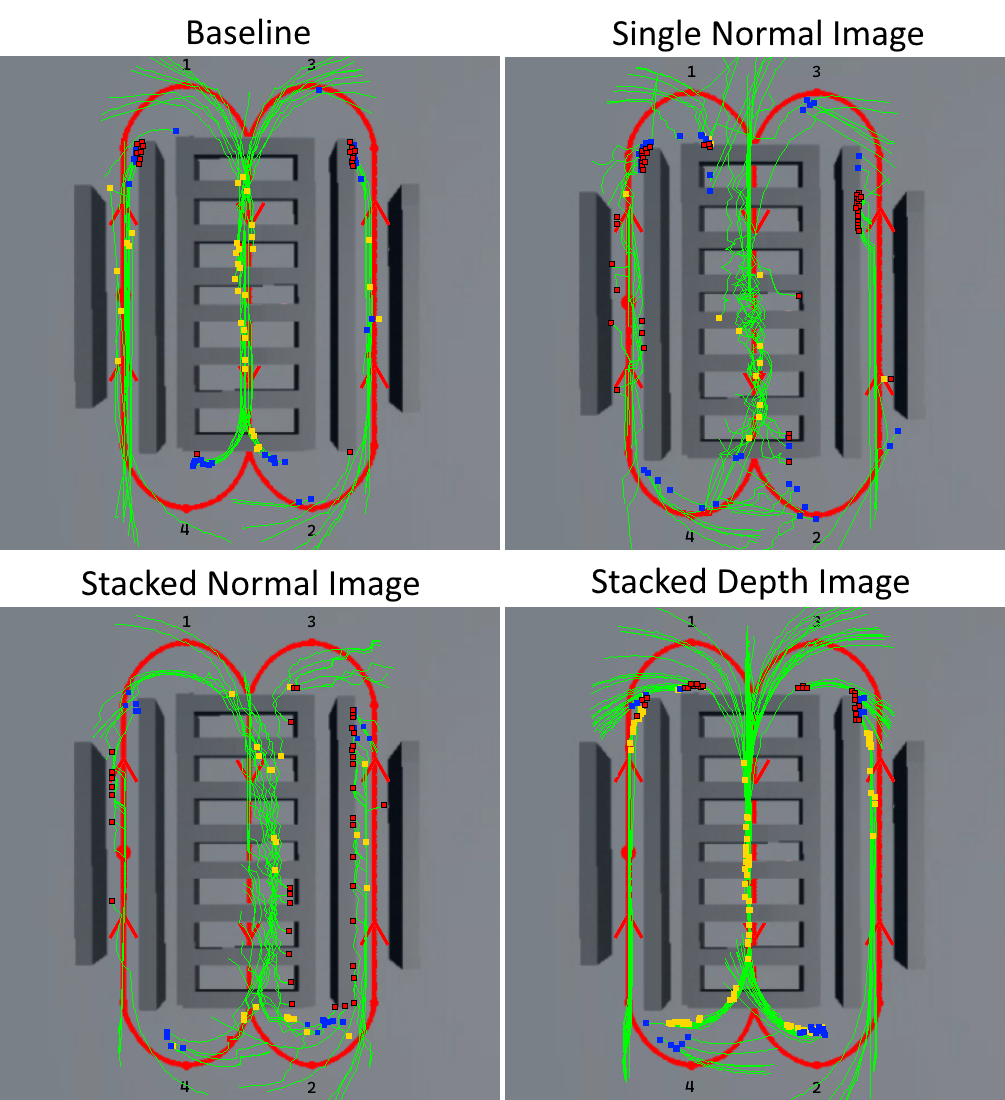
\includegraphics[width=0.66\linewidth]{results/summary-BlocksObstacles-PathsNew.png}
    \captionof{figure}[Overview of paths in BlocksObstacles environment]{Overview of paths in BlocksObstacles environment\newline\newline\newline\newline\newline\newline\newline\newline\newline\newline\newline\newline\newline\newline\newline\newline\newline
    The dots correspond to the following episode ends: \newline
    Red = Collisions\newline
    Blue = Out of View \newline
    Yellow = Corners}
    \label{im:ObstaclePaths}
\end{SCfigure}



\begin{SCfigure}
    \centering
    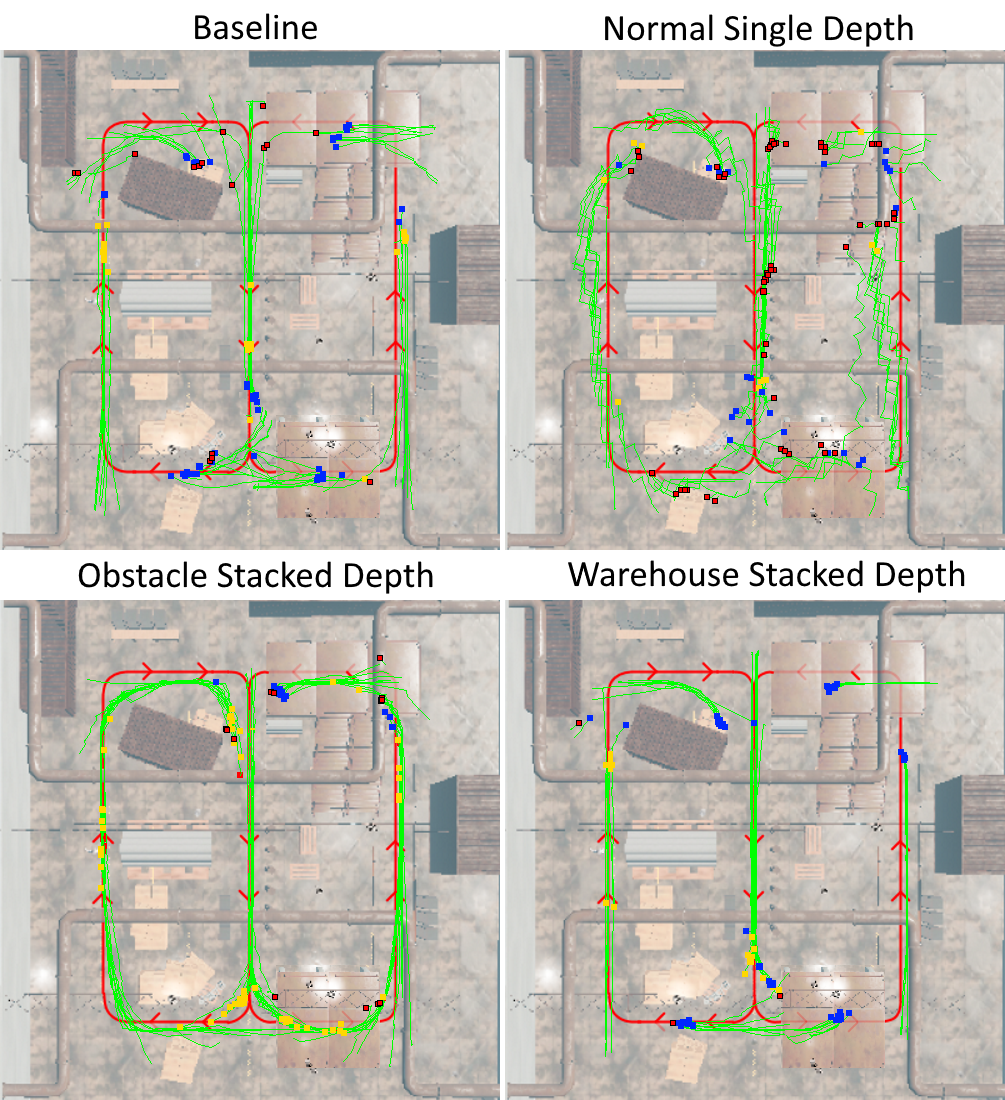
\includegraphics[width=0.66\linewidth]{results/WarehousePaths.png}
    \captionof{figure}[Overview of paths in Warehouse environment]{Overview of paths in Warehouse environment\newline\newline\newline\newline\newline\newline\newline\newline\newline\newline\newline\newline\newline\newline\newline\newline\newline\newline
    The dots correspond to the following episode ends: \newline
    Red = Collisions\newline
    Blue = Out of View \newline
    Yellow = Corners}
    \label{im:FactoryPaths}
\end{SCfigure}


